\subsection*{\databaseName{}}\label{subsec:evaluation-db}
% SQL vs NoSQL
According to \citeauthor{flask_book2018}, \ac{sql} databases are a good choice for efficiently storing structured data.
This is because their paradigm \acs{acid}, i. e. \acl{acid}, provides high reliability.
\ac{nosql} databases, on the other hand, are more flexible and can be used to store unstructured data \cite{flask_book2018}.
They do not require a predefined schema and can therefore accept documents of arbitrary structure \cite{flask2018}.
Usually, \ac{nosql} databases do not offer services such as \texttt{JOIN} \cite{flask2018}.
%According to \citeauthor{flask2018}, \ac{nosql} databases make a tradeoff between storage and speed, as well as a tradeoff between consistency and availability.
\ac{nosql} databases are said to outperform out-of-the-box \ac{sql} databases \cite{flask2018}.
Since the dataset consists of unstructured documents and the task at hand does not require performing any \texttt{JOIN}s a \ac{nosql} database is favourable.
\databaseName{} is chosen since it is well known to provide near real-time search and to operate on big data.
Subsequently, it is a good fit for the underlying dataset.

% separation of initialisation and insertion
The time necessary to perform the steps of filling the \databaseName{} database has been evaluated and improved throughout this work.
The current time measurements are shown in \autoref{fig:time_init_db}.
Portioning the work with the database is beneficial since it is possible to update the embeddings without having to recreate the database.
Moreover, modulizing the initialization and filling of the database facilitates debugging and comparing the models used to create the embeddings.

\begin{figure}[!htb] % htp = hier (h), top (t), oder auf einer eigenen Seite (p).
    \centering
    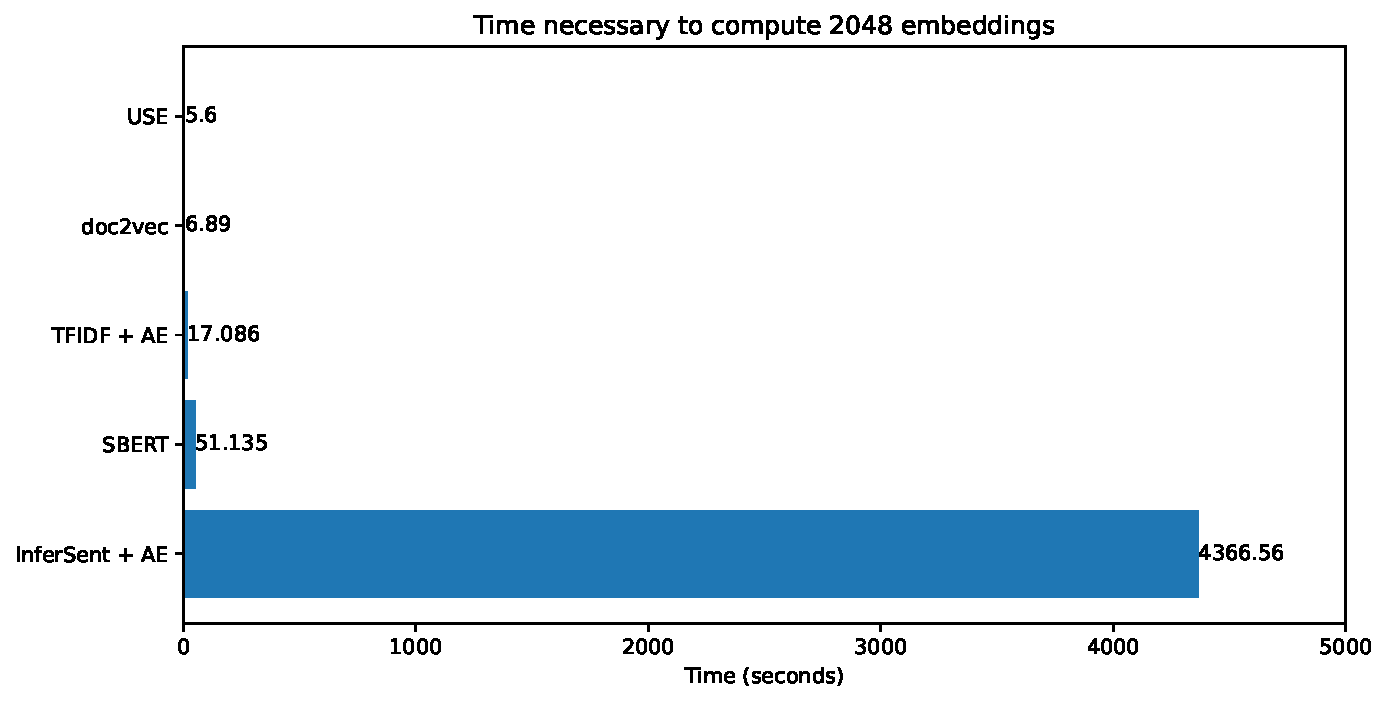
\includegraphics[width=1\textwidth]{images/Elasticsearch/Time_necessary_to_compute_2048_embeddings.pdf}
    \caption[Times for creating the database]{Time per module of creating the Bahamas database using a random selection of 2048 documents.
    The reference time is measured using \texttt{cProfiler} on a \localMaschineStats{}.
    %the \texttt{timer} from \texttt{timeit.default\_timer} on a \localMaschineStats{}.
    }
    \label{fig:time_init_db}
\end{figure}

%A document store database can be used if the primary goal is to write fast rather than write save \cite{flask2018}.